\part{Curvas}

\chapter{Curvas en el espacio}

En este capítulo daremos una introducción a la teoría de curvas en en el
espacio. Una curva representará el viaje emprendido por algún móvil $\alpha$
(una partícula o una mosca, por ejemplo) en el espacio $\R^3$.  Así, en cada
tiempo $t$, el móvil $\alpha$ se ubicará en el punto $\alpha(t)\in\R^3$. Esta
interpretación sugiere que una curva sea una función $\alpha$ con valores en
$\R^3$. Es natural pedir que $\alpha$ sea una función continua, pero esta
hipótesis no resulta del todo conveniente ya que las funciones continuas pueden
resultar bastante poco intuitivas. Para evitar patologías pediremos entonces
que nuestras curvas sean funciones de clase $C^\infty$. 

\begin{definition}
	\index{Curva!diferenciable}
	Una \textbf{curva diferenciable} es una función $\alpha\colon I\to\R^3$ de
	clase $C^{\infty}$, donde $I=(a,b)\subseteq\R$ es un intervalo abierto de
	$\R$.
\end{definition}

Entenderemos a un intervalo abierto en un sentido amplio, digamos $I=(a,b)$,
donde $a\in\R\cup\{-\infty\}$ y $b\in\R\cup\{+\infty\}$.  \index{Curva!vector
tangente a una} \index{Curva!velocidad de una} En este curso toda \emph{curva}
será una curva diferenciable. Si $\alpha\colon I\to\R^3$ es una curva
diferenciable, digamos $\alpha(t)=(x(t),y(t),z(t))$, las funciones coordenadas
$x$, $y$ y $z$ también son de clase $C^{\infty}$.  El vector
\[
	\alpha'(t)=(x'(t),y'(t),z'(t))
\]
es el \textbf{vector tangente} a $\alpha$ en el punto $\alpha(t)$. El vector
$\alpha'(t)$ también se denomina el vector velocidad de $\alpha$. 
\index{Vector!tangente a una curva}
\index{Vector!velocidad de una curva}

En la definición anterior utilizamos implícitamente la siguiente convención: una función
se dice \emph{diferenciable} si es de clase $C^{\infty}$.

\begin{example}
	Si $\alpha\colon\R\to\R^2$, $\alpha(t)=(t,|t|)$, entonces $\alpha$ no es
	una curva diferenciable ya que la función $t\mapsto |t|$ no es de clase
	$C^{\infty}$. Sin embargo, $\beta(t)=(t^3,|t|t^2)$ sí es una curva
	diferenciable y las imágenes de $\alpha$ y $\beta$ coinciden. La traza de
	estas curvas puede verse en la figura~\ref{fig:abs}.
	\begin{figure}
		\centering
    	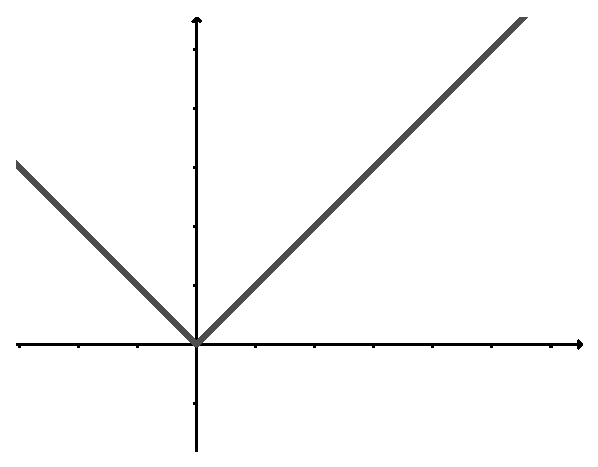
\includegraphics[scale=0.5]{eps/abs}
		\caption{¿Es este gráfico la traza de una curva diferenciable?}
		\label{fig:abs}
	\end{figure}
\end{example}

Es evidente que la curva del ejemplo anterior presenta una particularidad en el
origen. Más adelante explicaremos este fenómeno mediante el concepto de
regularidad de una curva.

\begin{definition}
	\index{Curva!plana}
	Una curva $\alpha\colon I\to\R^3$ se dice \textbf{plana} si existe un plano
	$P\subseteq\R^3$ tal que $\alpha(t)\in P$ para todo $t\in I$.
\end{definition}

Después de aplicar una traslación y una rotación conveniente, 
toda curva plana puede pensarse como una curva
$\alpha\colon I\to\R^3$ tal que $\alpha(t)=(x(t),y(t),0)$. Esta observación nos
permitirá tratar a nuestras curvas planas como curvas de la forma $\alpha\colon
I\to\R^2$. 

\begin{example}
	Una curva no tiene por qué ser inyectiva. 
	Si $\alpha(t)=(t^3-4t,t^2-4)$ es la curva de la figura~\ref{fig:not_injective}, 
	entonces $\alpha(2)=\alpha(-2)=(0,0)$.
	\begin{figure}
		\centering
    	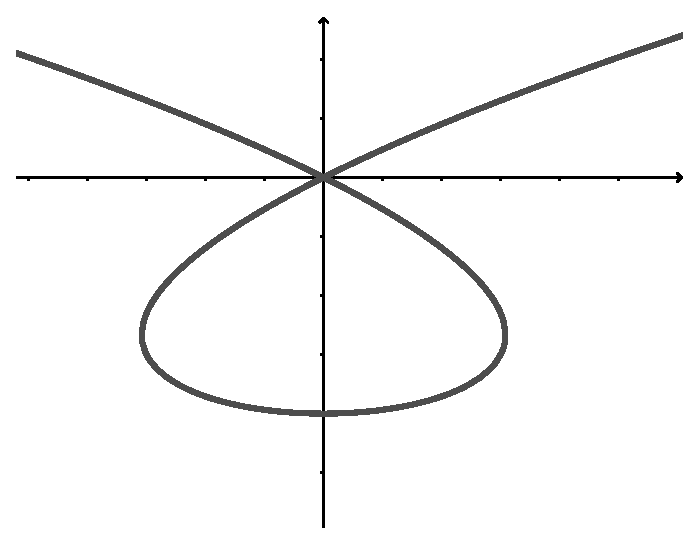
\includegraphics[scale=0.5]{eps/notinjective}
		\caption{Una curva no tiene por qué ser inyectiva.}
		\label{fig:not_injective}
	\end{figure}
\end{example}

\begin{example}
	Si $\alpha$ es una curva, su imagen puede tener picos. 
	Si $\alpha\colon\R\to\R^2$, $\alpha(t)=(t^3,t^2)$, entonces $\alpha(\R)$ es el gráfico de la función
	$x\mapsto x^{2/3}$, ver figura~\ref{fig:picos}.
	\begin{figure}
		\centering
    	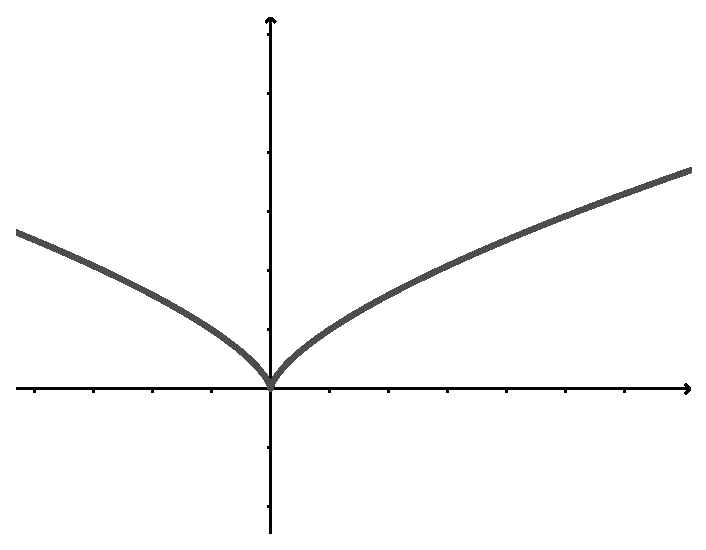
\includegraphics[scale=0.5]{eps/cups}
		\caption{Una curva podría tener picos.}
		\label{fig:picos}
	\end{figure}
\end{example}

\begin{example}
	En general $\alpha\colon I\to\alpha(I)$ no es un homeomorfismo, ni siquiera en
	el caso en que $\alpha$ sea inyectiva.
	Sea $\alpha\colon(-1,+\infty)\to\R^2$,
	$\alpha(t)=\left(\frac{3t}{1+t^3},\frac{3t^2}{1+t^3}\right)$.
	\begin{figure}
		\centering
    	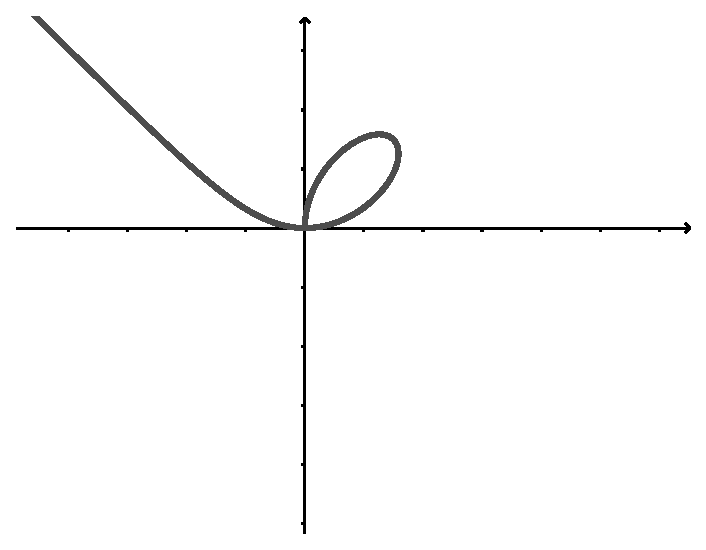
\includegraphics[scale=0.5]{eps/not}
		\caption{Folium de Descartes. Esta curva no es un homeomorfismo con su imagen.}
	\end{figure}
\end{example}

Veamos ahora ejemplos de curvas no planas. 
Los tres ejemplos siguientes resultarán fundamentales:

\begin{example}
	\label{Recta}
	Sean $p\in\R^3$ y $v\in\R^3$. La \textbf{recta} que pasa por $p$ y tiene dirección
	$v$ es una curva: $\alpha(t)=p+tv$.
\end{example}

\begin{example}
	\index{Círculo}
	Sean $p\in\R^3$ y $r>0$. El \textbf{círculo} con centro en $p$ y radio $r$ es una curva:
	$\alpha(t)=p+r(\cos(t/r),\sin(t/r))$. 
\end{example}

\begin{example}
	\index{Hélice circular}
	\label{exa:helice}
	Sean $a,b\in\R_{>0}$. La curva $\alpha\colon\R\to\R^3$, 
	\[
	\alpha(t)=\left(a\cos\frac{t}{\sqrt{a^2+b^2}},a\sin\frac{t}{\sqrt{a^2+b^2}},\frac{bt}{\sqrt{a^2+b^2}}\right),
	\]
	se conoce como
	\textbf{hélice circular} y puede verse en la figura~\ref{fig:helice}.
	\begin{figure}
		\centering
    	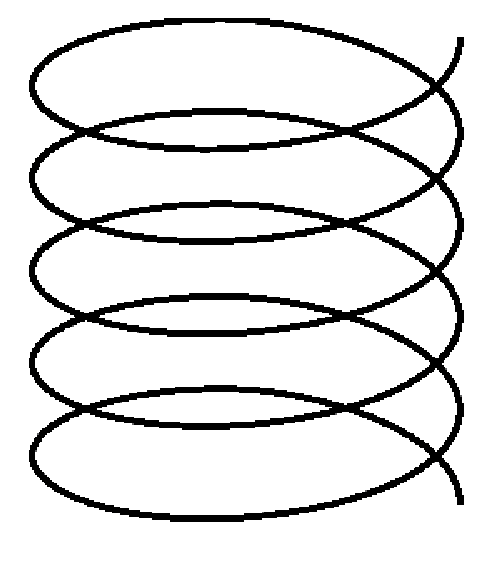
\includegraphics[scale=0.3]{eps/helix}
		\caption{La hélice circular.}
		\label{fig:helice}
	\end{figure}
\end{example}

Intentaremos a continuación definir la longitud de una curva $\alpha\colon
I\to\R^3$.  Intruitivamente es claro que la longitud de una cierta curva puede
aproximarse por la longitud de una poligonal que comparta algunos puntos con la
curva.  Sea entonces $[a,b]\subseteq I$ y sea $P$ una partición del intervalo
$[a,b]$. Recordemos que $P$ es un conjunto de puntos
\[
	a=t_0<t_1<\cdots<t_n=b.
\]
Definimos entonces la longitud de $\alpha$ en $[a,b]$ con respecto a $P$ como
\[
	L_a^b(\alpha,P)=\sum_{i=1}^n\|\alpha(t_i)-\alpha(t_{i-1})\|.
\]
Se define además el tamaño de la partición $P$ como el número 
\[
	|P|=\max_{1\leq i\leq n}|t_i-t_{i-1}|.
\]
Puede demostrarse que 
\[
	\lim_{|P|\to 0}L_a^b(\alpha,P)=\int_a^b\|\alpha'(t)|dt,
\]
y esto justifica la siguiente definición:

%\begin{theorem}
%	Para cada $\epsilon>0$ existe $\delta>0$ tal que si $|P|<\delta$, entonces 
%	\[
%		\left|L_a^b(\alpha,P)-\int_a^b\|\alpha'(t)\|dt\right|<\epsilon.
%	\]
%\end{theorem}
%
%\begin{proof}
%	Sea $f\colon I\times I\times I\to\R$ dada por
%	\[
%		f(t_1,t_2,t_3)=\sqrt{x'(t_1)^2+y'(t_2)^2+z'(t_3)^2}.
%	\]
%	Como la función $f$ es continua, es uniformemente continua en el compacto
%	$[a,b]$. Si $\epsilon>0$, existe $\delta>0$ tal que si $(t_1,t_2,t_3)$ y
%	$(s_1,s_2,s_3)$ son puntos de $[a,b]^3$ tales que $|t_i-s_i|<\delta$ para
%	todo $i\in\{1,2,3\}$, entonces
%	\[
%		|f(t_1,t_2,t_3)-f(s_1,s_2,s_3)|<\frac{\epsilon}{b-a}.
%	\]
%	Por el teorema del valor medio sabemos que existen
%	$\beta_i,\gamma_i,\delta_i\in [t_i,t_{i-1}]$ tales que
%	\[
%		\|\alpha(t_i)-\alpha(t_{i-1})\|=f(\beta_i,\gamma_i,\delta_i)(t_i-t_{i-1})
%	\]
%	Entonces
%	\[
%		L_a^b(\alpha,P)=\sum_{i=1}^n f(\beta_i,\gamma_i,\delta_i)(t_i-t_{i-1}).
%	\]
%	Por otro lado, si usamos el teorema del valor medio para integrales,
%	sabemos que existen $\xi_i\in(t_{i-1},t_i)$ tales que 
%	\begin{equation}
%		\label{eq:Lab}
%		\begin{aligned}
%			\int_a^b\|\alpha'(t)\|dt
%			&=\sum_{i=1}^n\int_{t_{i-1}}^{t_i}\|\alpha'(t)\|dt\\
%			&=\sum_{i=1}^n\|\alpha'(\xi_i)\|(t_i-t_{i-1})
%			=\sum_{i=1}^nf(\xi_i,\xi_i,\xi_i)(t_i-t_{i-1}).
%		\end{aligned}
%	\end{equation}
%	Si $P$ es tal que $|P|<\delta$, entonces $t_i-t_{i-1}<\delta$ para todo
%	$i\in\{1,\dots,n\}$. En particular, como
%	$t_{i-1}<\beta_i,\gamma_i,\delta_i<t_i$ para todo $i\in\{1,\dots,n\}$,
%	entonces $|\beta_i-\xi_i|<\delta$, $|\gamma_i-\xi|<\delta$ y 
%	$|\delta_i-\xi_i|<\delta$ para todo $i\in\{1,\dots,n\}$.  Luego 
%	\begin{align*}
%		\left|L_a^b(\alpha,P)-\int_a^b\|\alpha'(t)\|dt\right|
%		&\leq\sum_{i=1}^n|f(\beta_i,\gamma_i,\delta_i)-f(\xi_i,\xi_i,\xi_i)|(t_i-t_{i-1})\\
%		&<\frac{\epsilon}{b-a}\sum_{i=1}^n(t_i-t_{i-1})=\epsilon.	
%		\qedhere
%	\end{align*}
%\end{proof}

\begin{definition}
	\index{Curva!longitud de una}
	Sea $\alpha\colon I\to\R^3$ una curva y sean $a,b\in I$. Se define la
	\textbf{longitud} de $\alpha$ entre $a$ y $b$ como el número
	\[
		L_a^b(\alpha)=\int_a^b\|\alpha'(t)\|dt.
	\]
\end{definition}

%\index{Isometría}
%Una \textbf{isometría} de $\R^3$ es una función
%$\varphi\colon\R^3\to\R^3$ tal que 
%\[
%\|x-y\|=\|\varphi(x)-\varphi(y)\|
%\]
%para todo $x,y\in\R^3$. Es sabido que salvo una traslación $\varphi$ es una
%transformación lineal ortogonal, es decir cuya matriz asociada $A$ satisface
%$AA^T=I$.

\begin{definition}
	\index{Difeomorfismo}
	Sean $I$ y $J$ intervalos abiertos.  Un \textbf{difeomorfismo} entre $J$ e
	$I$ es una función inversible $\varphi\colon J\to I$ de clase $C^{\infty}$
	con inversa de clase $C^{\infty}$.
\end{definition}

\index{Reparametrización!de una curva}
Si $\alpha\colon I\to\R^3$ es una curva y $\varphi\colon J\to I$ es un
difeomorfismo, podemos construir una nueva curva $\beta\colon J\to\R^3$,
$\beta=\alpha\circ\varphi$. La curva $\beta$ es lo que se conoce como una
\textbf{reparametrización} de $\alpha$. Veamos cómo se comporta la longitud de
una curva con respecto a reparametrizaciones:

\begin{proposition}
	Sea $\varphi\colon J\to I$ un difeomorfismo y sea $\alpha\colon I\to\R^3$
	una curva. Si $[a,b]\subseteq J$ y $\varphi([a,b])=[c,d]$, entonces
	$L_a^b(\alpha\circ\varphi)=L_c^d(\alpha)$. 
\end{proposition}

\begin{proof}
	Por la regla de la cadena, 
	\[
		\|(\alpha\circ\varphi)'(t)\|=\|\alpha'(\varphi(t))\||\varphi'(t)|.
	\]
	Como $\varphi$ es un difemorfismo y $\varphi'(t)\ne0$ para todo $t$, tenemos que 
	$\varphi'>0$ o bien que $\varphi'<0$. Si $\varphi'(t)>0$ para todo $t$, entonces
	\[
		\int_a^b\|(\alpha\circ\varphi)'(t)\|dt=\int_a^b\|\alpha'(\varphi(t))\||\varphi'(t)|dt=\int_c^d\|\alpha'(s)\|ds.
	\]
	En caso de que $\varphi'<0$ la cuenta es similar. 
\end{proof}


\begin{definition}
	\index{Curva!regular}
	Una curva $\alpha\colon I\to\R^3$ se dice \textbf{regular} si
	$\|\alpha'(t)\|\ne 0$ para todo $t\in I$.
\end{definition}

Círculos y líneas son curvas regulares. 

\begin{example}
	La curva $\alpha(t)=(t^3,t^2)$ no es regular ya que $\alpha'(0)=(0,0)$.
	Vimos la imagen de esta curva en la figura~\ref{fig:picos}.
\end{example}

Queremos definir invariantes geométricos de una curva. Estos invariantes no
dependerán de la parametrización sino de las propiedades geométricas de la
curva. Nos convendrá entonces elegir, entre las muchas parametrizaciones
existentes, alguna que sea, en algún sentido, la mejor posible.

\begin{definition}
	\index{Curva!parametrizada por longitud de arco}
	\index{Curva!de rapidez unitaria}
	Sea $\alpha\colon I\to\R^3$ una curva. Se dice que $\alpha$ está
	\textbf{parametrizada por longitud de arco} si $\|\alpha'(t)\|=1$ para todo
	$t\in I$.
\end{definition}

A las curvas parametrizadas por longitud de arco también se las denomina
\textbf{curvas de rapidez unitaria}.

\begin{theorem}
	Toda curva regular puede parametrizarse por longitud de arco.
\end{theorem}

\begin{proof}
	Si $\alpha\colon I\to\R^3$ es una curva y $t_0\in I$, definimos
	\[
		s\colon I\to\R,\quad
		t\mapsto\int_{t_0}^t\|\alpha'(u)\|du=L_{t_0}^t(\alpha).
	\]

	Como la función $u\mapsto \|\alpha'(u)\|$ es continua, $s$ es una función diferenciable 
	tal que $s'(t)=\|\alpha'(t)\|$. Como $\|\alpha'(t)\|\ne 0$
	para todo $t$, $s\colon I\to s(I)$ es un difeomorfismo. En particular $s$
	es inversible. Sea $\varphi$ la inversa de $s$ y sea $J=s(I)$. Si 
	\[
		\beta(s)=(\alpha\circ\varphi)(s)\colon J\to\R^3,
	\]
	entonces
	\[
		\beta'(s)=\alpha'(\varphi(s))\varphi'(s)=\frac{\alpha'(\varphi(s))}{\|\alpha'(\varphi(s))\|}
	\]
	y luego $\|\beta'(s)\|=1$ para todo $s\in J$. 
\end{proof}

\begin{remark}
	La función $s$ no es única pues depende de $t_0$ y de una constante de
	integración.
\end{remark}

Veamos algunos ejemplos:

\begin{example}
	Sea $v$ un vector no nulo de $\R^3$ y $p\in\R^3$.  Si $\alpha(t)=tv+p$,
	entonces $\alpha'(t)=v$.  Como $s(t)=\int_0^t\|v\|du=t\|v\|$, se concluye
	que $\varphi(s)=s/\|v\|$ y luego
	\[
		\beta(s)=\frac{v}{\|v\|}s+p.
	\]
\end{example}

\begin{example}
	Sea $a>0$ y $b\ne0$. La curva $\alpha\colon\R\to\R^3$, $\alpha(t)=(a\cos
	t,a\sin t,bt)$, es regular pues $\alpha'(t)=(-a\sin t,a\cos t,b)\ne
	(0,0,0)$. Parametricemos $\alpha$ por longitud de arco. Primero calculamos
	$\|\alpha'(t)\|=\sqrt{a^2+b^2}$ y luego 
	\[
		s(t)=\int_0^t \sqrt{a^2+b^2}du=\sqrt{a^2+b^2}t.
	\]
	Tenemos entonces que $\varphi(s)=s/\sqrt{a^2+b^2}$ y luego 
	\[
		\beta(s)=\alpha(s/\sqrt{a^2+b^2})
		=\left(a\cos\frac{s}{\sqrt{a^2+b^2}},a\sin\frac{s}{\sqrt{a^2+b^2}},\frac{bs}{\sqrt{a^2+b^2}}\right).
	\]
\end{example}

\chapter{Las fórmulas de Frenet}

Comenzaremos por ver qué pasa en el caso de curvas planas. 

Sea entonces
$\alpha\colon I\to\R^2$ una curva plana parametrizada por longitud de arco. Escribamos $\alpha(s)=(x(s),y(s))$ y 
para cada $s\in I$ definamos 
\[
	T(s)=\alpha'(s)=(x'(s),y'(s)).
\]
La función $T\colon I\to\R^2$ es entonces diferenciable y además $\|T(s)\|=1$
para todo $s\in I$. Sea $N\colon I\to\R^2$ la función diferenciable dada por 
\[
	N(s)=(-y'(s),x'(s)).
\]
Entonces $\|N(s)\|=1$ y además $\langle T(s),N(s)\rangle=0$ para todo $s\in I$.
En particular, $\{T(s),N(s)\}$ es una base de $\R^2$ tal que 
\[
	\det(T(s),N(s))=1
\]
para todo $s\in I$; esta base se conoce como \textbf{diedro de Frenet} y nos
dice qué tanto se tuerce la curva $\alpha$. Sea $\kappa\colon I\to\R^2$ la
función diferenciable dada por
\[
	\kappa(s)=\langle T'(s),N(s)\rangle.
\]
La función $\kappa$ es la \textbf{curvatura} de $\alpha$.

Al derivar 
\[
	\langle T(s),T(s)\rangle=\|T(s)\|^2=1,\quad
	\langle N(s),N(s)\rangle=\|N(s)\|^2=1,\quad
	\langle T(s),N(s)\rangle=0,
\]
obtenemos que
\[
	T'(s)=\kappa(s)N(s),\quad
	N'(s)=-\kappa(s)T(s).
\]

\begin{example}
	Sea $\alpha(s)=r(\cos(s/r),\sin(s/r))$ el círculo con centro en $(0,0)$ y
	radio $r>0$. Observemos que $\alpha$ está parametrizada por longitud de arco. 
	Un cálculo directo muestra que
	\begin{align*}
	T(s)&=\alpha'(1)=(-\sin(s/r),\cos(s/r)),\\
	T'(s)&=(1/r)(-\cos(s/r),-\sin(s/r)),\\
	N'(s)&=(-\cos(s/r),-\sin(s/r)).
	\end{align*}
	Luego $\kappa(s)=\langle T'(s),N(s)\rangle=1/r$. 
\end{example}

Veamos qué pasa si en el ejemplo anterior cambiamos la orientación de la curva. 

%\begin{proposition}
%	Sea $\alpha\colon I\to\R^2$ una curva plana. Entonces
%	\[
%		T'(s)=\kappa(s)N(s),\quad
%		N'(s)=-\kappa(s)t(s).
%	\]
%\end{proposition}

Veamos ahora una construcción análoga para curvas espaciales. 

Sea $\alpha$ una curva parametrizada por longitud de arco. Si
$T(s)=\alpha'(s)$, entonces $\|T(s)\|=1$ para todo $s$. Además $T$ es ortogonal a
$T$ pues, como $\langle T(s),T(s)\rangle=1$ para todo $s$, al derivar obtenemos
que $\langle T'(s),T(s)\rangle=0$ pues
\[
	\langle T'(s),T(s)\rangle+\langle T(s),T'(s)\rangle=0.
\]

\index{Curvatura!de una curva}
La \textbf{curvatura} de $\alpha$ en $s$ es 
la función 
\[
\kappa(s)=\|T'(s)\|.
\]
Nuestra definición de curvatura implica que $\kappa(s)\geq0$ para todo $s$,
algo que no pasa en el caso de curvas planas. 

En general solamente podemos asegurar que $\kappa$ es una función continua. Si
$T'(s)\ne 0$ para todo $s$, entonces $\kappa$ es una función de clase
$C^{\infty}$. 

De ahora en adelante supondremos que $\kappa(s)>0$ para todo $s$. 

\index{Vector normal!a una curva}
El \textbf{vector normal} a $\alpha$ en $s$ se define como la función $N\colon I\to\R^3$ dada por 
\[
N(s)=\frac{T'(s)}{\|T'(s)\|}=\kappa(s)^{-1}T'(s).
\]
De la definición se tiene que $N$ es diferenciable y que 
\[
	\langle N(s),N(s)\rangle=1,\quad
	\langle T(s),N(s)\rangle=0
\]
para todo $s\in I$.

\index{Vector!binormal a una curva}
Por último, el \textbf{vector binormal} a $\alpha$ en $s$ se define como la
función
\[
	B(s)=T(s)\times N(s),
\]
donde $T(s)\times N(s)$ denota al producto vectorial entre $T(s)$ y $N(s)$. 

\begin{definition}
	\index{Triedro de Frenet}
	La base de $\R^3$ formada por $T(s)$, $N(s)$ y $B(s)$ se conoce como el triedro de Frenet.
\end{definition}

\index{Torsión!de una curva}
Si derivamos $B(s)=T(s)\times N(s)$, obtenemos
\begin{align*}
	B'(s)=T'(s)\times N(s)+T(s)\times N'(s)=T(s)\times N'(s)
\end{align*}
pues $T'(s)=\kappa(s)N(s)$. Luego $\langle B'(s),T(s)\rangle=0$. Por otro lado,
al derivar la expresión $\langle B(s),B(s)\rangle=1$, obtenemos $\langle
B'(s),B(s)\rangle=0$. Luego existe $\tau(s)$ tal que $B'(s)=\tau(s)N(s)$. La
\textbf{torsión} de $\alpha$ en $s$ es el escalar $\tau(s)$. La función
$\tau\colon I\to\R$, $\tau(s)=\langle B'(s),N(s)\rangle$ es diferenciable.

\begin{theorem}
	Sea $\alpha\colon I\to\R^3$ una curva parametrizada por longitud de arco
	tal que $\kappa>0$. Entonces
	\begin{align*}
		T'=\kappa N, && 
		N'=-\kappa T-\tau B, && 
		B'=\tau N.
	\end{align*}
\end{theorem}

\begin{proof}
	La primera fórmula es consecuencia de la definición de 
	$N(s)$ y la tercera de la definición de $\tau(s)$. Al derivar
	la expresión
	$\langle N(s),T(s)\rangle=0$ 
	obtenemos
	\begin{align*}
		\langle N'(s),T(s)\rangle+\langle N(s),T'(s)\rangle
		&=\langle N'(s),T(s)\rangle+\langle N(s),\kappa(s)N(s)\rangle\\
		&=\langle N'(s),T(s)\rangle+\kappa(s)
	%	\langle N(s),T(s)\rangle=0=\langle N(s),B(s)\rangle,
	\end{align*}
	Similarmente al derivar $\langle N(s),B(s)\rangle=0$, 
	\[
		\langle N'(s),B(s)\rangle+\langle N(s),B'(s)\rangle=\langle N'(s),B(s)\rangle+\tau(s)=0.
	\]
	Luego 
	\[
	N'(s)=\langle N'(s),T(s)\rangle T(s)+\langle N'(s),B(s)\rangle B(s)=-\kappa(s)T(s)-\tau(s)B(s).\qedhere
	\]
\end{proof}

\index{Fórmulas de Frenet!para curvas en el espacio}
Las fórmulas del teorema anterior se conocen como las \textbf{fórmulas de Frenet}.

\begin{example}
	Si $\alpha(s)=sv+v_0$, con $\|v\|=1$, entonces $T(s)=v$ y $\kappa(s)=0$.
\end{example}

\begin{example}
	Sea $\alpha(s)=r\left(\cos(s/r),\sin(s/r),0\right)+c$ el círculo con centro en $c$ y radio $r>0$. 
	Calculamos
	\[
		\alpha'(s)=r\left(\frac{-1}{r}\sin(s/r),\frac{1}{r}\cos(s/r),0\right)=(-\sin(s/r),\cos(s/r),0),
	\]
	y entonces $\|\alpha'(s)\|=1$ para todo $s$. Esto nos dice que $T(s)=\alpha'(s)$. Calculamos ahora
	\[
		T'(s)=\left(\frac{-1}{r}\cos(s/r),\frac{-1}{r}\sin(s/r),0\right),
	\]
	y obtenemos que $\kappa(s)=\frac{1}{r}\ne0$. Como entonces
	$N(s)=(-\cos(s/r),-\sin(s/r),0)$ y $B(s)=(0,0,1)$, se concluye que
	$B'(s)=0$ y luego $\tau(s)=0$.
\end{example}

%En el ejercicio anterior vemos que si $b=0$, entonces $\tau=0$. Observar que en
%este caso, $\alpha$ resulta ser una curva plana. Esto motiva la siguiente
%interpretación de la torsión:
Veamos otra interpretación geométrica de la torsión:

\begin{proposition}
	Sea $\alpha$ una curva parametrizada por longitud de arco
	tal que $\kappa(s)>0$ para todo $s$. Entonces $\alpha$ es plana si y sólo si $\tau=0$.
\end{proposition}

\begin{proof}
	Supongamos primero que $\tau=0$. Como entonces $B'(s)=0$ para todo $s$,
	existe un vector $v\in\R^3$ tal que $B(s)=v$ para todo $s$. Veamos que
	$\alpha(s)$ pertenece al plano con vector normal $v$ que pasa por el punto
	$\alpha(0)$. Queremos demostrar entonces que
	$\langle \alpha(s)-\alpha(0),v\rangle=0$ para todo $s$. Sea $f(s)=\langle \alpha(s)-\alpha(0),v\rangle$. Como 
	\[
		f'(s)=\langle\alpha'(s),v\rangle=\langle T(s),B(s)\rangle=0
	\]
	y además $f(0)=0$, entonces 
	la función $f$ es contantemente igual a cero. 

	Sea $P$ un plano con vector normal $v\in\R^3$ y tal que $p\in P$ y supongamos que 
	$\alpha(s)\in P$ para todo $s$. Entonces $\langle\alpha(s)-p,v\rangle=0$
	para todo $s$. Al derivar dos veces esta expresión se obtiene
	\[
		\langle \alpha'(s),v\rangle=\langle\alpha''(s),v\rangle=0
	\]
	y luego $v$ es ortogonal a $\alpha'(s)=T(s)$ y también es ortogonal a
	$N(s)=\kappa(s)^{-1}\alpha''(s)$. Como entonces $v=\lambda B$ para algún
	$\lambda\in\R$, se concluye que $B(s)=\pm \frac{v}{\|v\|}$ es un vector
	constante. Esto implica que $B'(s)=0$ y luego $\tau(s)=0$. 
\end{proof}

Veamos otra interpretación:

\begin{proposition}
	Sea $\alpha$ una curva parametrizada por longitud de arco tal que su
	curvatura $\kappa(s)=\kappa$ es una constante positiva.  Si $\tau(s)=0$
	para todo $s$, entonces $\alpha$ es parte de una circunferencia de radio
	$1/\kappa$.
\end{proposition}

\begin{proof}
	Como $\tau(s)=0$ para todo $s$, la proposición anterior nos dice que
	$\alpha$ es una curva plana. Sea $\gamma(s)=\alpha(s)+\kappa^{-1}N(s)$. Si
	derivamos y usamos las fórmulas de Frenet obtenemos
	\[
		\gamma'(s)=\alpha'(s)+\kappa^{-1}N'(s)=T(s)+\kappa^{-1}(-\kappa T(s))=0.
	\]
	Esto implica que $\gamma(s)=c$ es una constante y entonces
	$\alpha(s)+\kappa^{-1}N(s)=c$ para todo $s$. Veamos ahora que todo punto de
	la curva dista en $\kappa^{-1}$ del punto $c$:
	\[
		\|\alpha(s)-c\|=\|\kappa^{-1}N(s)\|=\kappa^{-1}.\qedhere
	\]
\end{proof}

\chapter{El teorema fundamental}

Sea $\alpha\colon I\to\R^3$ una curva parametrizada por longitud de arco tal
que $\kappa>0$.  Las fórmulas de Frenet pueden escribirse matricialmente de la
siguiente forma:
\begin{align*}
	\colvec{3}{T'(s)}{N'(s)}{B'(s)}
	&=\begin{pmatrix}
		0 & \kappa(s)I_3 & 0\\
		-\kappa(s)I_3 & 0 & -\tau(s)I_3\\
		0 & \tau(s)I_3 & 0
	\end{pmatrix}
	\colvec{3}{T(s)}{N(s)}{B(s)},
\end{align*}
donde $I_3$ es la matriz identidad de $3\times 3$.

\begin{theorem}
	\index{Teorema!fundamental de curvas}
	Sean $\kappa_0\colon I\to\R$ una función positiva de clase $C^{\infty}$ y
	$\tau_0\colon I\to\R$ una función de clase $C^{\infty}$.  Existe entonces
	una curva $\alpha\colon I\to\R^3$
	parametrizada por longitud de arco tal que $\kappa(s)=\kappa_0(s)$ y
	$\tau_(s)=\tau_0(s)$ para todo $s$. 
\end{theorem}

\begin{proof}
	Consideremos la ecuación diferencial 
	\begin{equation}
		\label{eq:fundamental}
		X'(s)=A_0(s)X(s),\quad
		A_0(s)=\begin{pmatrix}
		0 & \kappa_0(s)I_3 & 0\\
		-\kappa_0(s)I_3 & 0 & -\tau_0(s)I_3\\
		0 & \tau_0(s)I_3 & 0
	\end{pmatrix}\in\R^{9\times 9},
\end{equation}
	donde $I_3$ denota la matriz identidad de $3\times 3$. 
	Sea $a\in\R^9$ tal que los vectores
	\[
		t_0=(a_1,a_2,a_3),\quad
		m_0=(a_4,a_5,a_6),\quad
		b_0=(a_7,a_8,a_9)
	\]
	forman una base orientada ortonormal de $\R^3$. Sea $f\colon I\to\R^9$ una
	solución de~\eqref{eq:fundamental} tal que $f(s_0)=a$, para algún $s_0\in I$
	fijo, y sean 
	\begin{align*}
		&t=(f_1,f_2,f_3), 
		&&n=(f_4,f_5,f_6),
		&&b=(f_7,f_8,f_9).
	\end{align*}
	Entonces
	\[
		t'(s)=\kappa_0(s)n(s),\quad
		n'(s)=-\kappa_0(s)t(s)-\tau_0(s)b(s),\quad
		b'(s)=\tau_0(s)n(s).
	\]
	Veamos que $\{t(s),n(s),b(s)\}$ es una base ortonormal de $\R^3$ para todo
	$s\in I$. Para cada $s\in I$ sea $M(s)$ la matriz 
	\[
		M(s)=\begin{pmatrix}
			\langle t(s),t(s)\rangle & \langle t(s),n(s)\rangle & \langle t(s),b(s)\rangle\\
			\langle n(s),t(s)\rangle & \langle n(s),n(s)\rangle & \langle n(s),b(s)\rangle\\
			\langle b(s),t(s)\rangle & \langle b(s),n(s)\rangle & \langle b(s),b(s)\rangle
		\end{pmatrix}.
	\]
	Como $M'(s)=A(s)M(s)-M(s)A(s)$, donde
	\[
		A(s)=\begin{pmatrix}
		0 & \kappa_0(s) & 0\\
		-\kappa_0(s) & 0 & -\tau_0(s)\\
		O & \tau_0(s) & 0
	\end{pmatrix},
	\]
	y además $M(s_0)=I_3$, el teorema de existencia y unicidad garantiza que
	$M(s)=I_3$ para todo $s\in I$. Luego $\{t(s),n(s),b(s)\}$ es una base
	ortonormal. Como, en particular, $\det(t(s),n(s),b(s))=\pm 1$ y
	$\det(t(s_0),n(s_0),b(s_0))=1$, la continuidad implica que
	$\det(t(s),n(s),b(s))=1$  y luego $\{t(s),n(s),b(s)\}$ es una base
	positivamente orientada.

	Sea $\alpha\colon I\to\R^3$ dada por 
	\[
		\alpha(s)=\int_{s_0}^st(u)du.
	\]
	Entonces $\alpha$ es una curva diferenciable tal que $T(s)=\alpha'(s)=t(s)$. En particular,
	$|T(s)|=|\alpha'(s)|=|t(s)|=1$ y luego $\alpha$ está parametrizada
	por longitud de arco. Además
	$\kappa(s)=|T'(s)|=|t'(s)|=\kappa_0(s)$ y 
	entonces $N(s)=n(s)$. Por último, 
	\[
		B(s)=T(s)\times N(s)=t(s)\times n(s)=b(s)
	\]
	y luego $\tau(s)=\tau_0(s)$ pues
	$\tau(s)n(s)=\tau(s)N(s)=B'(s)=b'(s)=\tau_0(s)n(s)$.
\end{proof}

Puede demostrarse que la curva $\alpha$ del teorema anterior es única salvo
movimientos rígidos. 

\chapter{La desigualdad isoperimétrica}

\index{Curva!simple}
\index{Curva!cerrada}
En esta sección nos concentraremos en curvas planas simples y cerradas. Diremos
que una curva plana $\alpha$ es \textbf{cerrada} si $\alpha\colon I\to\R^2$,
donde $I=[a,b]$, es tal que $\alpha(a)=\alpha(b)$. Además $\alpha$ es
\textbf{simple} si $\alpha$ no tiene autointersecciones.

\begin{example}
	Sean $p,q\in\R_{>0}$. 
	La elipse $\alpha\colon [0,2\pi]\to\R^2$, $\alpha(t)=(p\cos t,q\sin t)$, es
	una curva simple y cerrada. El interior 
	\[
		\inner\alpha=\{(x,y)\in\R^2:(x/p)^2+(y/q)^2<1\}
	\]
	de $\alpha$ es una región acotada y el exterior 
	es 
	\[
		\ext\alpha=\{(x,y)\in\R^2:(x/p)^2+(y/q)^2>1\}
	\]
	es una región no acotada. 
	\begin{figure}
		\centering
    	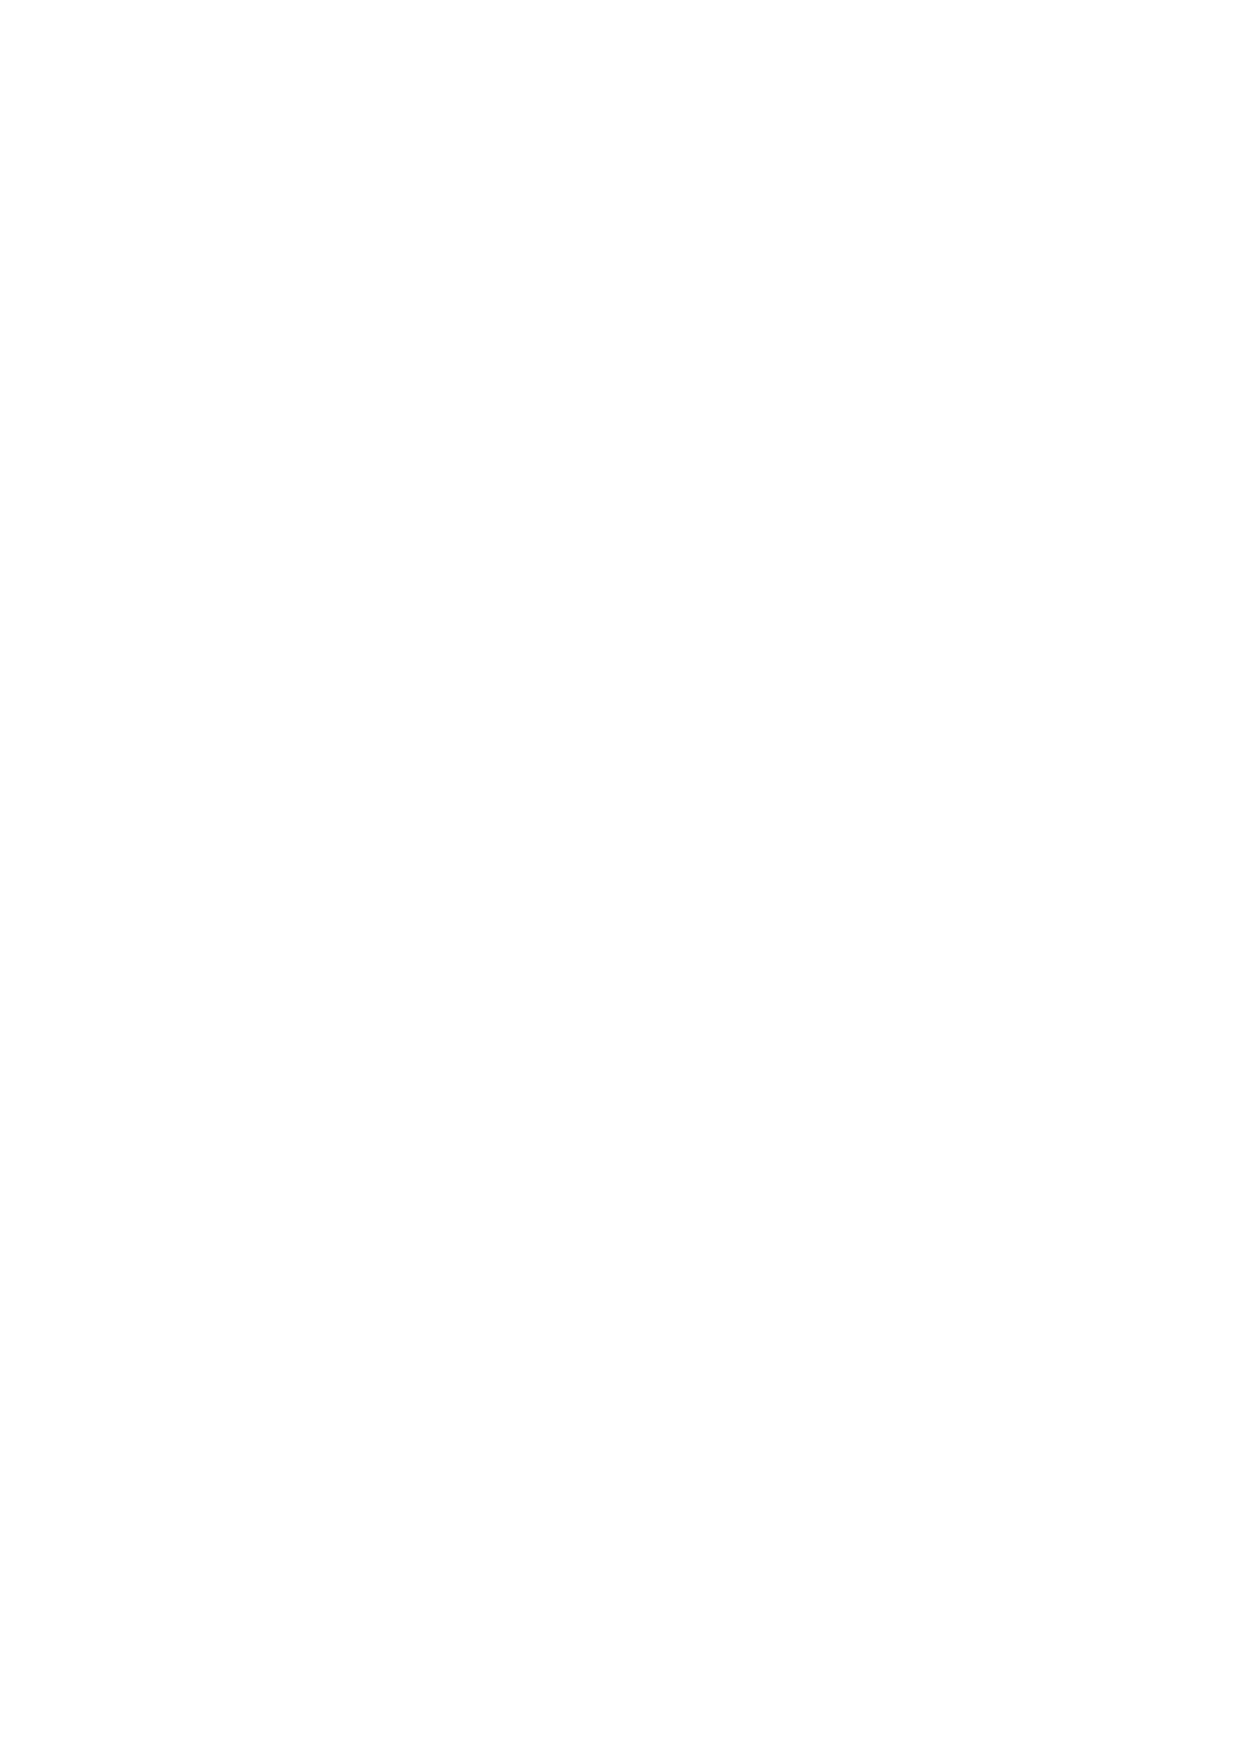
\includegraphics[scale=0.05]{eps/elipse}
		\caption{La elipse con $p=5$ and $q=2$.}
		\label{fig:elipse}
	\end{figure}
\end{example}

\begin{example}
	La curva $\alpha(t)=( (1+2\cos t)\cos t,(1+2\cos t)\sin t)$ que vemos en la
	figura~\ref{fig:self} es cerrada pero no es simple ya que tiene
	autointersecciones: $\alpha(2\pi/3)=\alpha(4\pi/3)$. 
	\begin{figure}
		\centering
    	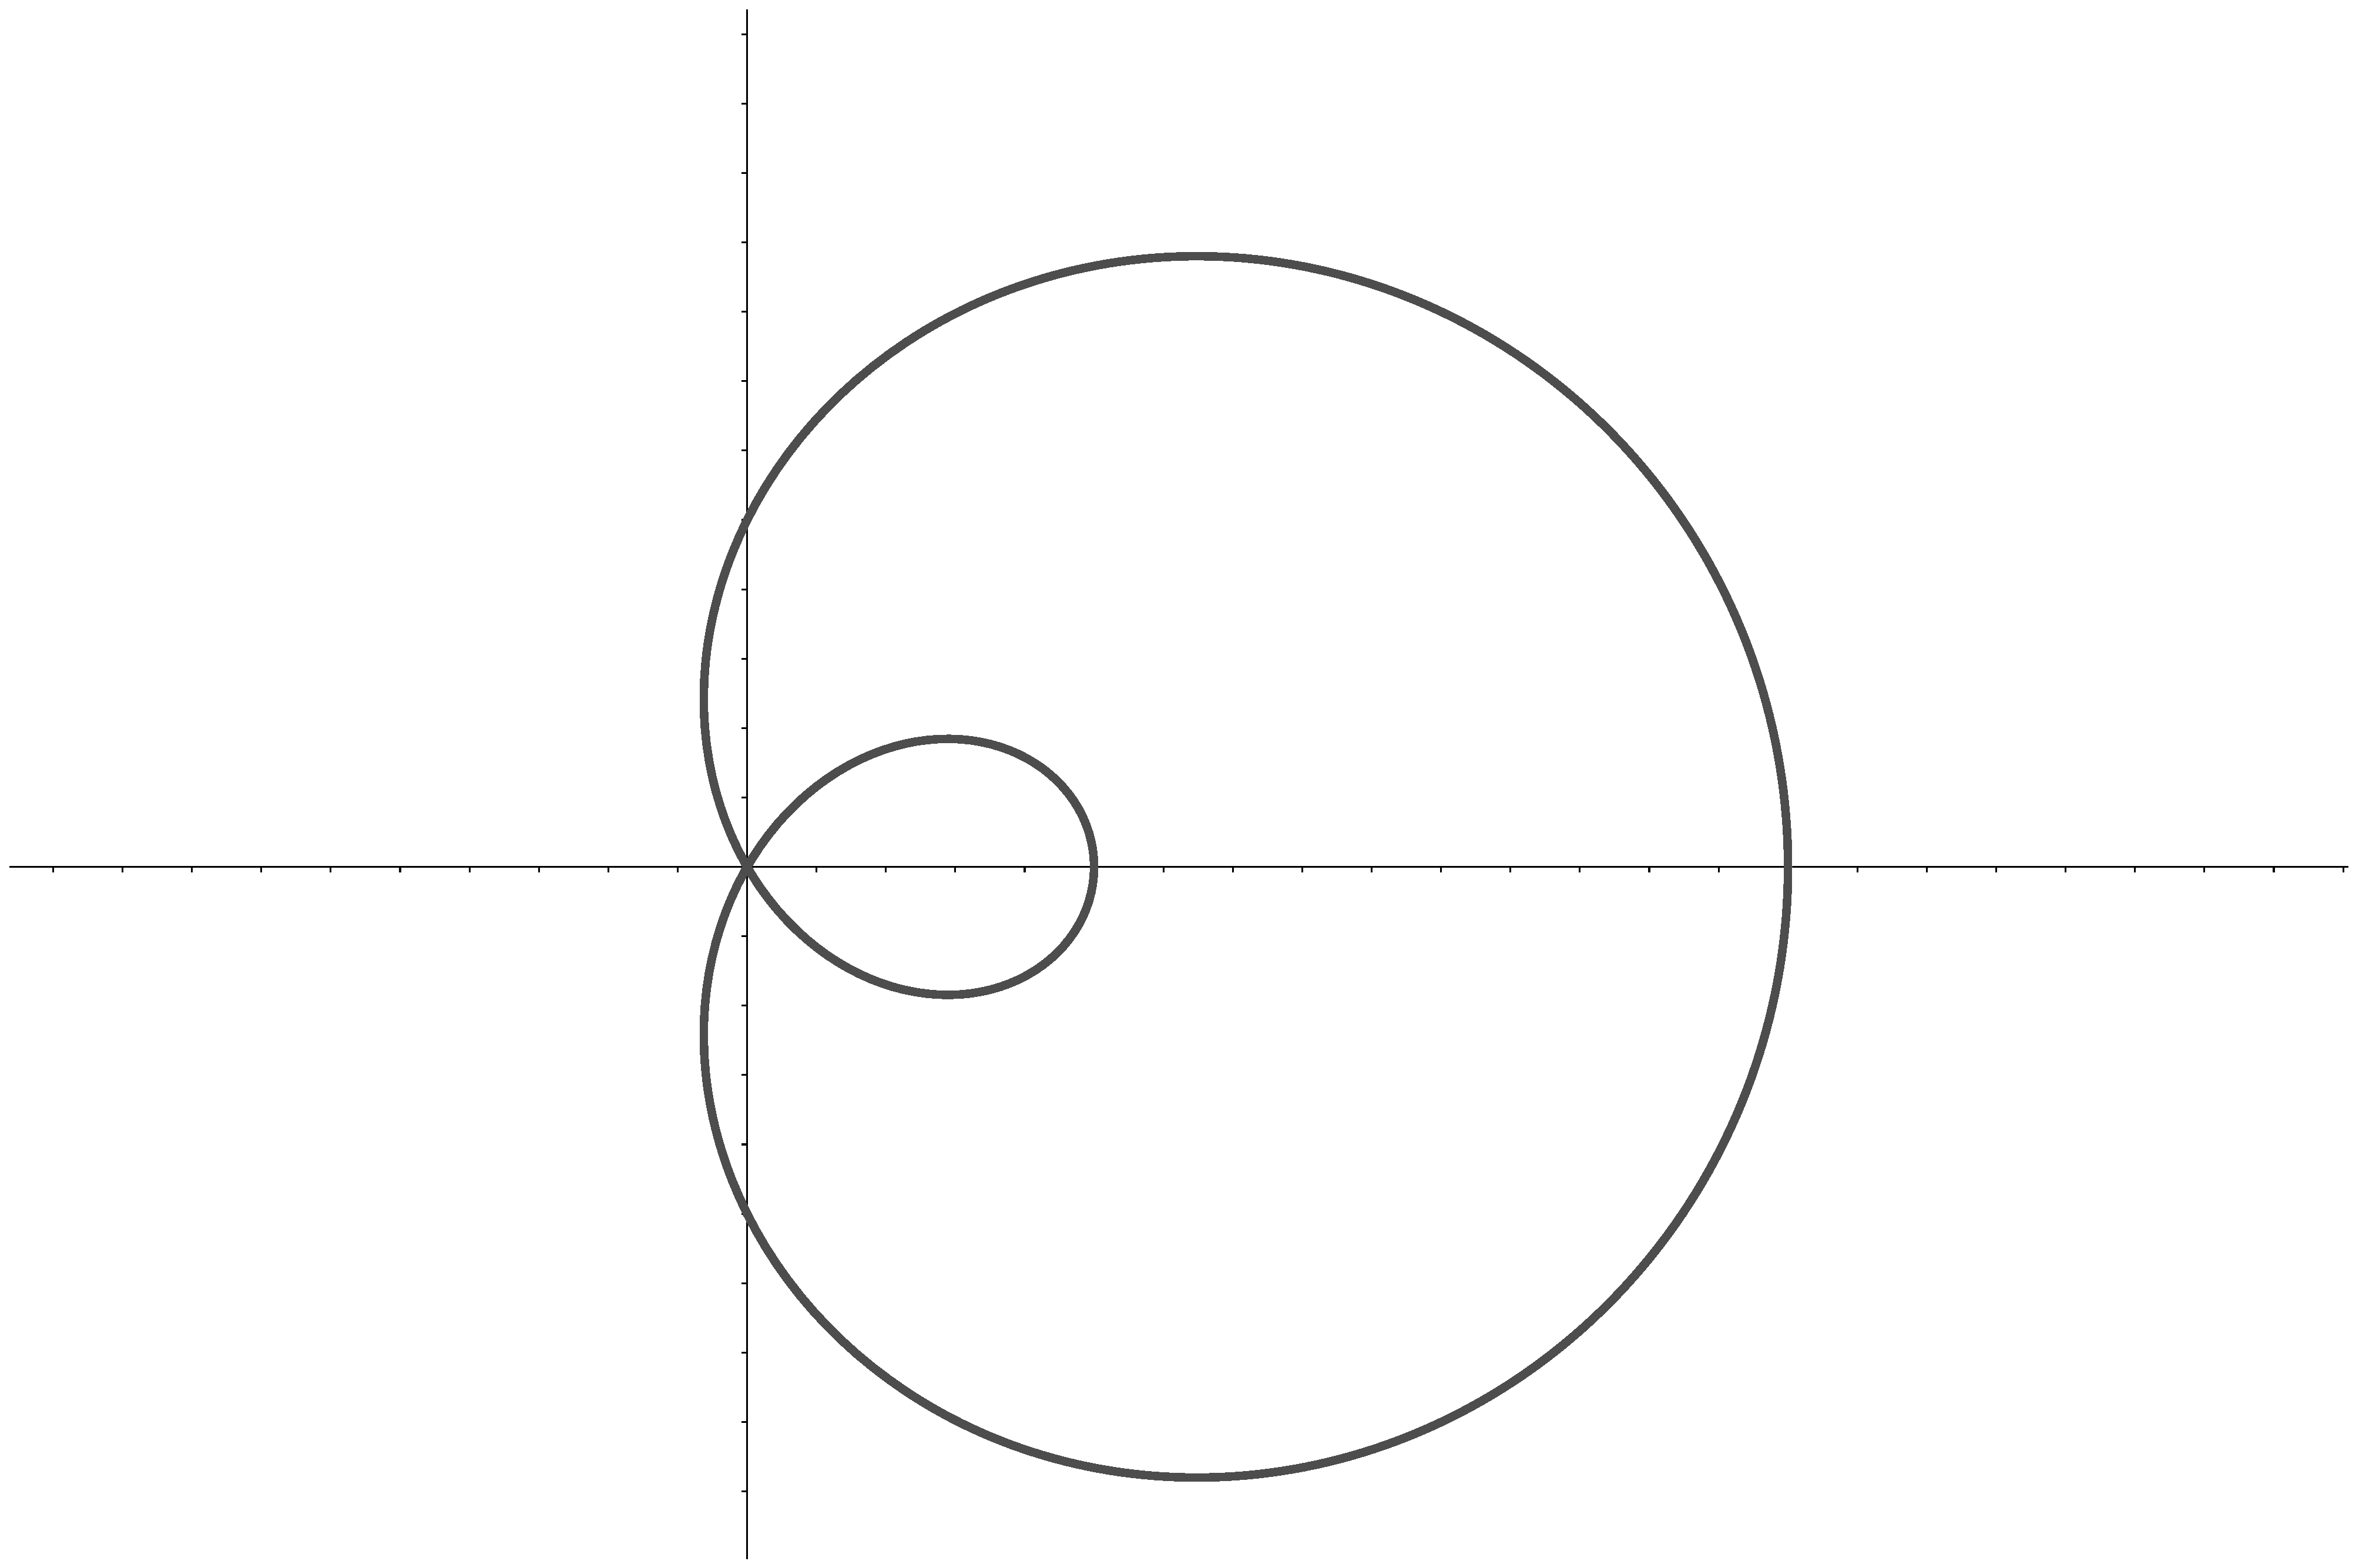
\includegraphics[scale=0.1]{eps/self}
		\caption{Una curva cerrada y no simple.}
		\label{fig:self}
	\end{figure}
\end{example}

\index{Teorema!de la curva de Jordan}
El \textbf{teorema de Jordan} afirma que toda curva simple y cerrada divide al
plano en dos regiones de las cuales una es acotada y la otra no. Más
precisamente, si $\alpha$ es una curva simple y cerrada, entonces
$\R^2\setminus\alpha=\inner\alpha\cup\ext\alpha$ (unión disjunta), donde el
interior $\inner\alpha$ de $\alpha$ es una región acotada y conexa y el
exterior $\ext\alpha$ de $\alpha$ es una región no acotada y conexa. La figura~\ref{fig:Jordan} 
nos muestra por qué el teorema de Jordan no es algo obvio.

El teorema de Jordan nos permite orientar una curva simple y cerrada: diremos
que nuestra curva $\alpha$ está orientada positivamente si en cada punto
$\alpha(t)$ normal apunta hacia el interior de $\alpha$.

\begin{figure}[H]
		\centering
    	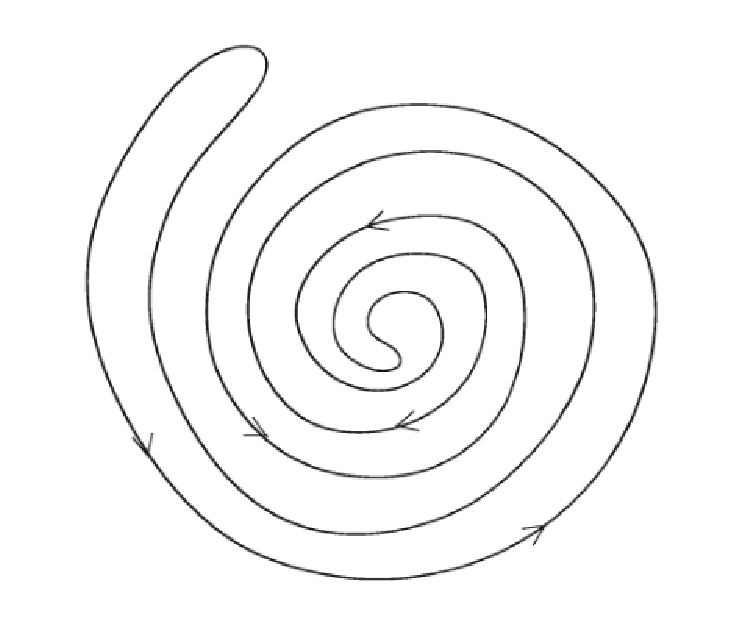
\includegraphics[scale=0.5]{eps/jordan}
		\caption{El teorema de Jordan no es una trivialidad.} 
		\label{fig:Jordan}
\end{figure}

\index{Problema isoperimétrico}
El problema isoperimétrico es el siguiente. Entre todas las curvas planas
simples y cerradas de una longitud dada, queremos encontrar la curva que acote
la región con mayor área.	
Para resolver el problema isopetrimétrico necesitamos recordar el
\textbf{teorema de Green}. Si $R$ es la región acotada dentro de una curva
simple y cerrada $\alpha$ de $\R^2$ y $f,g\colon\R^2\to\R$ son funciones
diferenciables, entonces
\[
	\int_{\inner\alpha}\left(\frac{\partial g}{\partial x}-\frac{\partial f}{\partial y}\right)dxdy
	=\int_\alpha f(x,y)dx+g(x,y)dy.
	%\left(f\frac{dx}{dt}+g\frac{dy}{dt}\right)dt.
\]
Si en el teorema de Green $f(x,y)=-y$ y $g(x,y)=x$, entonces se obtiene la
siguiente fórmula:
\[
	2\text{área}(R)=\int_a^b\left( x(t)\frac{dy}{dt}-y(t)\frac{dx}{dt}\right)dt
\]

\index{Desigualdad!de Cauchy--Schwarz}
Otra de la herramientas que necesitamos para resolver el problema
isopetrimétrico es la \textbf{desigualdad de Cauchy--Schwarz}: si $v,w\in\R^n$,
entonces 
\[
|\langle v,w\rangle|\leq\|v\|\|w\|.
\]
Más aún, vale la igualdad si y
sólo si $v=\lambda w$ para algún $\lambda\in\R$.

\begin{theorem}
	\index{Desigualdad!isopetrimétrica}
	Sea $\alpha$ una curva plana simple y cerrada de longitud $L$ y sea $R$ 
	la región encerrada por $\alpha$. Entonces
	\[
		\text{área}(R)\leq \frac{L^2}{4\pi}.
	\]
\end{theorem}

\begin{proof}
	Supongamos que la curva $C$ está parametrizada por longitud de arco,
	digamos $\alpha(s)=(x(s),y(s))$, $s\in[0,L]$. 
	El área de la región $R$ encerrada por $\alpha$ puede
	calcularse como
	\[
		\text{área}(R)=\frac12\int_0^L(xy'-yx')(s)ds.%=\int_0^Lx(s)y'(s)ds.
	\]
	Como $\alpha$ es una curva cerrada, 
	\begin{align*}
		\int_0^Lx(s)y'(s)ds&=\int_0^L((xy)'(s)-x'(s)y(s))ds\\
		&=(xy)(L)-(xy)(0)-\int_0^Lx'(s)y(s)ds=-\int_0^L x'(s)y(s)ds,
	\end{align*}
	y en consecuencia 
	\[
		\text{área}(R)=\int_0^Lx(s)y'(s)ds.
	\]
	Consideremos ahora el círculo $Z$ con centro en el origen y radio $r$
	parametrizado por $\beta(s)=(x(s),z(s))$.  El área del círculo $Z$ es
	\[
		\pi r^2=-\int_0^Lx'(s)z(s)ds.
	\]
	Al usar la desigualdad de Cauchy--Schwarz con los vectores $v=(x(s),-z(s))$
	y $w=(y'(s),x'(s))$ obtenemos 
	\begin{equation}
	\label{eq:isopetrimetrica1}
	\begin{aligned}
		\text{área}(R)+\pi r^2&=\int_0^L(x(s)y'(s)-z(s)x'(s))ds\\
		%&\leq\int_0^L\sqrt{(x(s)y'(s)-z(s)x'(s))^2}ds\\
		&\leq\int_0^L\sqrt{x(s)^2+z(s)^2}\sqrt{x'(s)^2+y'(s)^2}ds\\
		&=\int_0^L\sqrt{x(s)^2+z(s)^2}\\
		&=rL
	\end{aligned}
	\end{equation}
	pues $\alpha$ está parametrizada por longitud de arco. 
	Al usar la desigualdad 
	$\frac{a+b}{2}\geq \sqrt{ab}$ con $a=\text{área}(R)$ y $b=\pi r^2$ se obtiene que 
	$2\sqrt{\text{área}(R)}\sqrt{\pi r^2}\leq \text{área(R)}+\pi r^2\leq rL$. 
	Luego 
	\begin{equation}
		\label{eq:isoperimetrica2}
	4\pi r^2\text{área}(R)\leq r^2L^2,
	\end{equation}
	que es equivalente a la
	desigualdad que queriamos demostrar.
\end{proof}

Puede demostrarse que la igualdad en el teorema anterior vale si y sólo si
$C$ parametriza un círculo.

%\begin{exercise}
%	\label{xca:isoperimetrica}
%	Demuestre que en el teorema anterior vale la igualdad si y sólo si $C$
%	parametriza un círculo.	
%\end{exercise}

\chapter{Ejercicios}

\begin{exercise}
	\label{xca:L_t}
	Sea $C$ el círculo de radio $1$ con centro en $(0,0)$. Para cada $t\in\R$
	sea $L_t$ la recta de pendiente $t$ que pasa por el punto $(-1,0)$. La
	recta $L_t$ corta a $C$ en un cierto punto $\alpha(t)$. Encuentre una
	fórmula para $\alpha(t)$ que no use funciones trigonométricas y demuestre
	que $\alpha$ es una curva cuya imagen es $C\setminus\{(-1,0)\}$.
\end{exercise}

\begin{exercise}
	\label{xca:minima_distancia}
	Demuestre que si $\alpha\colon I\to\R^3$ es una curva y $[a,b]\subseteq I$,
	entonces 
	\[
		\|\alpha(b)-\alpha(a)\|\leq L_a^b(\alpha).
	\]
\end{exercise}

\begin{exercise}
	\label{xca:espiral_log}
	Dados $a>0$ y $b<0$, sea $\alpha\colon\R\to\R^2$ 
	la \textbf{espiral logarítmica}, ver figura~\ref{fig:log_spiral}. Esta curva 
	está dada por 
	\[
		\alpha(t)=(ae^{bt}\cos(t),ae^{bt}\sin(t)).
	\]
	Si $t_0=0$, demuestre que $s(t)=\frac{e^{bt}-1}{b}a(b^2+1)^{1/2}$. 
	\begin{figure}
		\centering
    	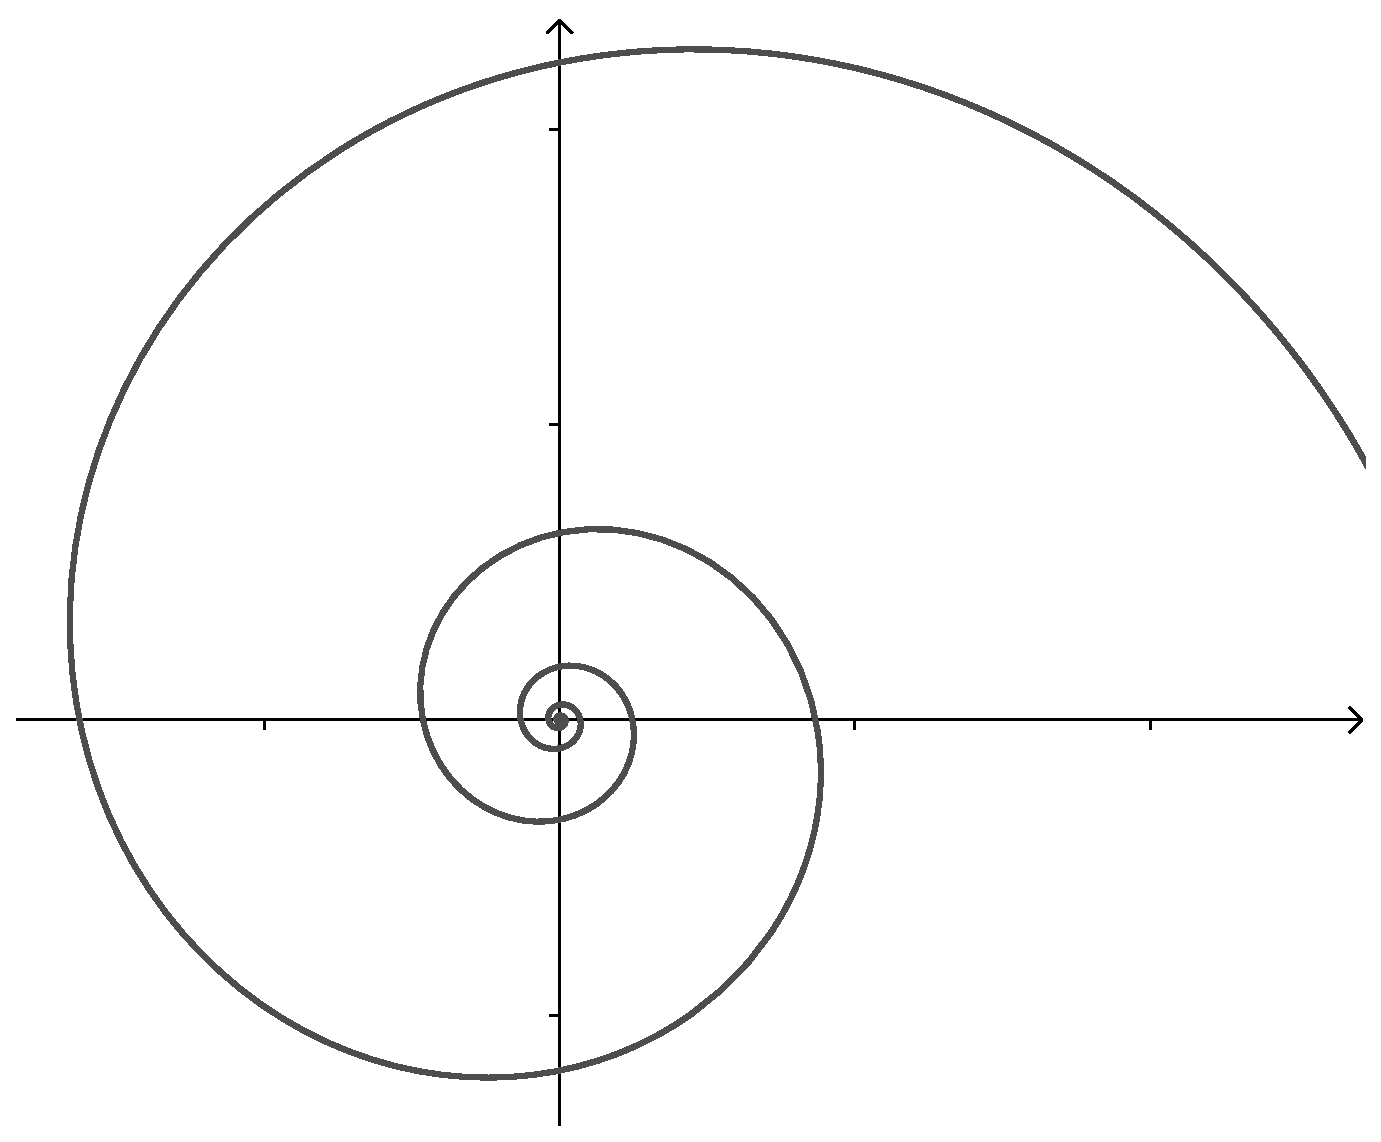
\includegraphics[scale=0.25]{eps/logspiral}
		\caption{La espiral logarítmica.}
		\label{fig:log_spiral}
	\end{figure}
%	\begin{align*}
%		s(t)=\int_0^t\left|\left(a(be^{bt}\cos t-e^{bt}\sin t),a(be^{by}\sin t+e^{bt}\cos t)\right)|dt
%	\end{align*}
\end{exercise}

\begin{exercise}
	\label{xca:circle}
	Sea $\alpha(s)=r(\cos(s/r),-\sin(s/r))$. Demuestre que 
	$\kappa(s)=-1/r$.
\end{exercise}

\begin{exercise}
	\label{xca:t=0}
	Sea 
	\[
		\alpha\colon\R\to\R^3,
		\quad
		\alpha(t)=\left(\frac{1}{\sqrt{3}}\cos t+\frac{1}{\sqrt{2}}\sin t,\frac{1}{\sqrt{3}}\cos t,\frac{1}{\sqrt{3}}\cos t-\frac{1}{\sqrt{2}}\sin t\right).
	\]
	Verifique que $\alpha$ está parametrizada por longitud de arco y calcule la
	curvatura y la torsión.	
\end{exercise}

\begin{exercise}
	\label{xca:helice}
	Demuestre que si $\alpha$ es la hélice circular del
	ejemplo~\ref{exa:helice}, entonces 
	\[
	\kappa(s)=\frac{|a|}{a^2+b^2},\quad
	\tau(s)=\frac{-b}{a^2+b^2}.
	\]
\end{exercise}

\begin{exercise}
	\label{xca:curvatura}
	Demuestre que la curvatura de una curva regular $\alpha$ puede calcularse
	como
	\[
		\kappa(t)=\frac{\|\alpha'\times\alpha''\|}{\|\alpha'\|^3}.
	\]
\end{exercise}

\begin{exercise}
	\label{xca:torsion}
	Demuestre que la torsión de una curva regular $\alpha$ 
	puede calcularse como
	\[
		\tau(t)=-\frac{\langle \alpha'\times\alpha'',\alpha'''\rangle}{\|\alpha'\times\alpha''\|^2}.
	\]
\end{exercise}

\begin{exercise}
	\label{xca:(t,t2,t3)}
	Calcule la curvatura y la torsión de la curva $\alpha(t)=(t,t^2,t^3)$. 
\end{exercise}

\begin{exercise}
	\label{xca:y=f(x)}
	Sea $f$ una función de clase $C^{\infty}$.  Calcule la curvatura y la
	torsión de la curva $\alpha(t)=(t,f(t),0)$. 
\end{exercise}


